\documentclass[tikz,border=5pt]{standalone}
\usepackage{amsmath,amssymb,fontspec,unicode-math}
\setmainfont{STIXTwoText-Regular.otf}
\setmathfont{STIXTwoMath-Regular.otf}
\usetikzlibrary{positioning,arrows.meta,calc,decorations.pathreplacing}
\begin{document}
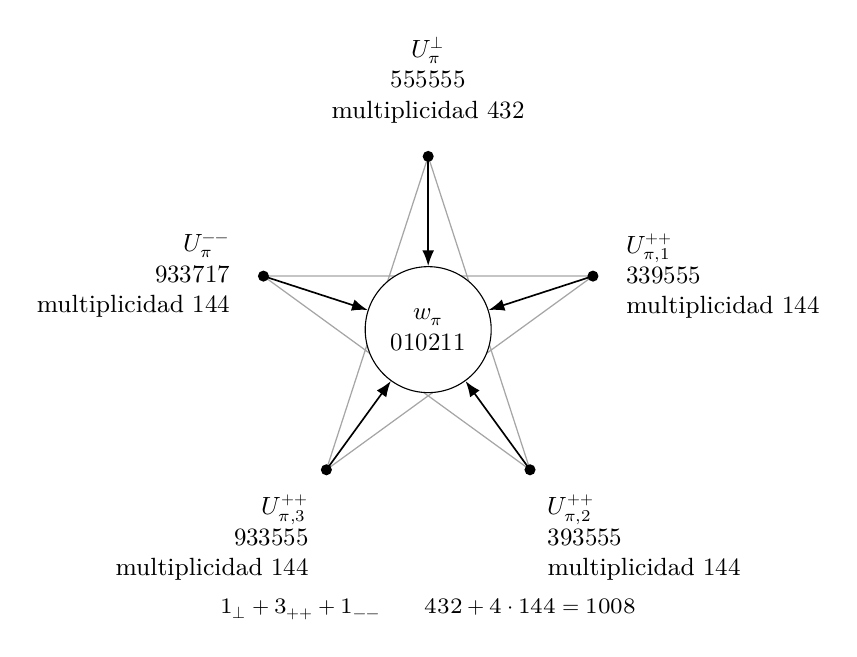
\begin{tikzpicture}[x=1cm,y=1cm,font=\small,>=Latex]
 \coordinate (a) at (90:2.2);
 \coordinate (b) at (18:2.2);
 \coordinate (c) at (-54:2.2);
 \coordinate (d) at (-126:2.2);
 \coordinate (e) at (162:2.2);
 \draw[black!35,line width=.45pt]
    (a)--(c)--(e)--(b)--(d)--cycle;
 \node[draw,fill=white,circle,minimum size=1.6cm,align=center,
    inner sep=3pt] (z) at (0,0) {$w_\pi$\\$010211$};
 \foreach \v in {a,b,c,d,e}{
    \fill (\v) circle (2pt);
    \draw[->,line width=.6pt] (\v)--(z);
 }
 \node[above=3mm,align=center] at (a)
   {$U_\pi^\perp$\\$555555$\\multiplicidad $432$};
 \node[right=3mm,align=left] at (b)
   {$U_{\pi,1}^{++}$\\$339555$\\multiplicidad $144$};
 \node[below right=2mm and 1mm,align=left] at (c)
   {$U_{\pi,2}^{++}$\\$393555$\\multiplicidad $144$};
 \node[below left=2mm and 1mm,align=right] at (d)
   {$U_{\pi,3}^{++}$\\$933555$\\multiplicidad $144$};
 \node[left=3mm,align=right] at (e)
   {$U_\pi^{--}$\\$933717$\\multiplicidad $144$};
 \node[align=center,font=\footnotesize] at (0,-3.55)
   {$1_\perp+3_{++}+1_{--}$\qquad $432+4\cdot144=1008$};
\end{tikzpicture}
\end{document}

